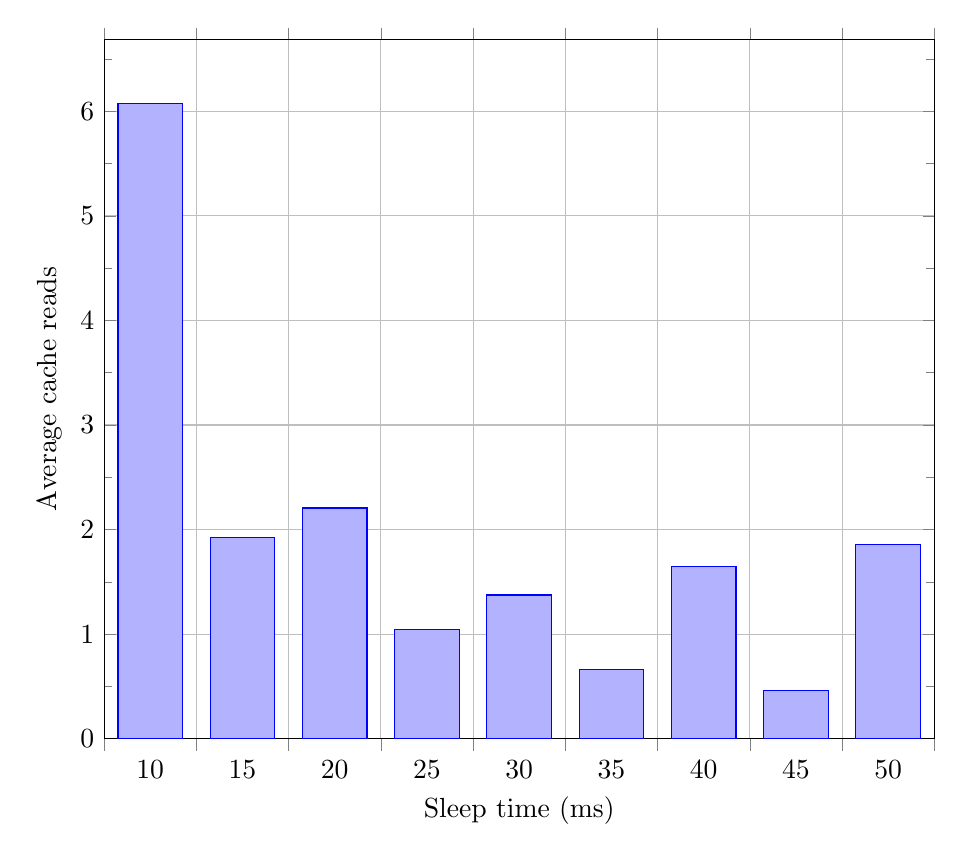
\begin{tikzpicture}
\begin{axis}
[
width=\resultsPlotWidthScale\textwidth,
%axis y line*=left,
xlabel=Sleep time (ms),
ymin = 0,
xmin = 10, xmax=55,
ylabel=Average cache reads,
%ymajorgrids=true,
%yminorgrids=true,
ybar interval=0.7,
ymajorgrids=true,
minor y tick num=1
%minor tick num=1
]


\addplot coordinates {
	(10 ,6.076278918444858)
	(15 ,1.9250837336102817)
	(20 ,2.206446850393701)
	(25 ,1.044688862465319)
	(30 ,1.3747593094220163)
	(35 ,0.661782154722354)
	(40 ,1.6464805561590268)
	(45 ,0.46317152740208856)
	(50 ,1.858914282814271)
	(55 ,0)
};

%matlab info
%     General model:
%     f(x) = (a/(x+b))+ c
%     Coefficients (with 95% confidence bounds):
%     a =       7.017  (-8.781, 22.82)
%     b =      -8.622  (-11.55, -5.697)
%     c =      0.9821  (0.01249, 1.952)
     
%\addplot[
%red,
%domain=10:50,
%samples=201,
%]
%{(7.017/(x-8.622))+ 0.9821};

\end{axis}
\end{tikzpicture}